\documentclass[12pt,a4paper]{article}

% --- Packages de base ---
\usepackage[utf8]{inputenc}
\usepackage[T1]{fontenc}
\usepackage[french]{babel}
\usepackage{geometry}
\geometry{top=2.5cm, bottom=2.5cm, left=2.5cm, right=2.5cm}

% --- Typographie et mise en page ---
\usepackage{lmodern}
\usepackage{fancyhdr}
\usepackage{titlesec}
\usepackage{float}
\usepackage{graphicx}
\usepackage{xcolor}
\usepackage{listings}
\usepackage{hyperref}
\usepackage{amsmath}

% --- Configuration des liens hypertextes ---
\hypersetup{
    colorlinks=true,
    linkcolor=blue,
    filecolor=magenta,      
    urlcolor=cyan,
    pdftitle={Rapport de Projet - AR Assembly Guide},
    pdfpagemode=FullScreen,
}

% --- Couleurs personnalisées pour le code ---
\definecolor{codeblue}{rgb}{0.13, 0.13, 1.0}
\definecolor{codegreen}{rgb}{0, 0.5, 0}
\definecolor{codegray}{rgb}{0.46, 0.45, 0.48}
\definecolor{codepurple}{rgb}{0.58, 0, 0.82}
\definecolor{backgroundcolor}{rgb}{0.96, 0.96, 0.96}

% --- Configuration des listings pour C# ---
\lstset{
    language=[Sharp]C,
    backgroundcolor=\color{backgroundcolor},
    commentstyle=\color{codegreen},
    keywordstyle=\color{codeblue}\bfseries,
    numberstyle=\tiny\color{codegray},
    stringstyle=\color{codepurple},
    basicstyle=\ttfamily\small,
    breakatwhitespace=false,         
    breaklines=true,                 
    captionpos=b,                    
    keepspaces=true,                 
    numbers=left,                    
    numbersep=5pt,                  
    showspaces=false,                
    showstringspaces=false,
    showtabs=false,                  
    tabsize=4
}

% --- En-tête et Pied de page ---
\pagestyle{fancy}
\fancyhf{}
\lhead{Rapport de Projet - Réalité Augmentée}
\rhead{Guide d'Assemblage Interactif}
\cfoot{\thepage}
\renewcommand{\headrulewidth}{0.4pt}
\renewcommand{\footrulewidth}{0.4pt}

% --- Titre ---
\title{
    \vspace{1.5cm}
    \Huge \textbf{Rapport de Projet} \\
    \vspace{0.5cm}
    \LARGE \textbf{Guide d'Assemblage Assisté par Réalité Augmentée} \\
    \vspace{1.5cm}
    \large \textbf{Dépôt GitHub du Projet :} \\
    \url{https://github.com/nouhailasalahmi/AR-Assembly-Guide} \\
    \vspace{1.5cm}
    \large \textit{Application d'assistance industrielle interactive développée sous Unity 6 et Vuforia Engine}
    \vspace{2.5cm}
}
\author{\textbf{Nouhaila Salahmi}}
\date{\today}

\begin{document}

\maketitle
\thispagestyle{empty}
\newpage

\tableofcontents
\newpage

% =========================================================================
\section{Introduction et Contexte}
% =========================================================================
Dans les secteurs industriels de pointe, les opérations de montage mécanique requièrent une précision absolue et une concentration constante de la part des opérateurs. Les méthodes traditionnelles basées sur des manuels d'instruction papier ou des écrans statiques augmentent la charge cognitive et le risque d'erreur humaine.

La Réalité Augmentée (AR) apporte une réponse directe à cette problématique en superposant des instructions dynamiques tridimensionnelles sur l'environnement physique réel de l'opérateur. 

Le travail présenté dans ce rapport décrit la réalisation d'une application d'assistance interactive dédiée à l'assemblage pas-à-pas d'un mécanisme de moteur composé d'un **vilebrequin**, d'une **bielle** et d'un **piston**. Ce système s'appuie sur le moteur graphique **Unity 6** et le kit de développement **Vuforia Engine** pour le tracking d'objets, assurant une intégration fluide entre les composants physiques réels et les aides visuelles virtuelles.

Le code source complet, les scènes de travail et les configurations du projet sont disponibles sur le dépôt GitHub officiel : 
\begin{center}
    \url{https://github.com/nouhailasalahmi/AR-Assembly-Guide}
\end{center}

% =========================================================================
\section{Cahier des Charges et Objectifs du Travail}
% =========================================================================
L'objectif principal est de concevoir un système d'assistance complet capable de guider, valider et évaluer le travail de montage d'un opérateur sans intervention humaine externe. Le périmètre fonctionnel comprend :

\begin{enumerate}
    \item \textbf{La détection et le suivi spatial} : Suivre en temps réel la bielle, le piston et le vilebrequin grâce à des cibles d'images physiques distinctes.
    \item \textbf{Le guidage interactif séquentiel} : Charger les étapes de montage depuis une configuration externe dynamique (JSON) et afficher les instructions adéquates à chaque étape.
    \item \textbf{Le contrôle géométrique automatique} : Valider automatiquement ou manuellement le bon positionnement et la bonne orientation des pièces physiques par rapport aux cibles de montage définies avec des tolérances millimétriques et angulaires.
    \item \textbf{L'évaluation de la performance} : Évaluer la qualité du travail à travers un score d'efficacité sur 100 points, basé sur les erreurs de manipulation et le respect du temps alloué.
\end{enumerate}

% =========================================================================
\section{Conception Technique et Modélisation du Système}
% =========================================================================

\subsection{Modèle de Guidage Séquentiel (Machine à États)}
Pour garantir que l'opérateur réalise les tâches dans l'ordre chronologique requis, la logique applicative est modélisée sous la forme d'une machine à états finis. Les états suivants orchestrent le déroulement d'une session :
\begin{itemize}
    \item \textbf{Idle (Attente)} : Écran d'accueil affichant le nom de la procédure et le nombre d'étapes.
    \item \textbf{Running (Exécution)} : Phase active où l'opérateur doit positionner la pièce demandée. Les chronomètres et les vérifications de tolérance sont actifs.
    \item \textbf{Transitioning (Transition)} : Se déclenche dès qu'une étape est validée. Un feedback positif est affiché et l'étape suivante se prépare.
    \item \textbf{Completed (Terminé)} : Fin de la procédure. La machine calcule le score final et affiche le tableau de bord d'évaluation.
\end{itemize}

\subsection{Cibles de Suivi de Réalité Augmentée}
La détection tridimensionnelle utilise des marqueurs physiques spécifiques (*Image Targets*) configurés dans la base de données Vuforia du projet :
\begin{figure}[H]
    \centering
    \begin{minipage}{0.3\textwidth}
        \centering
        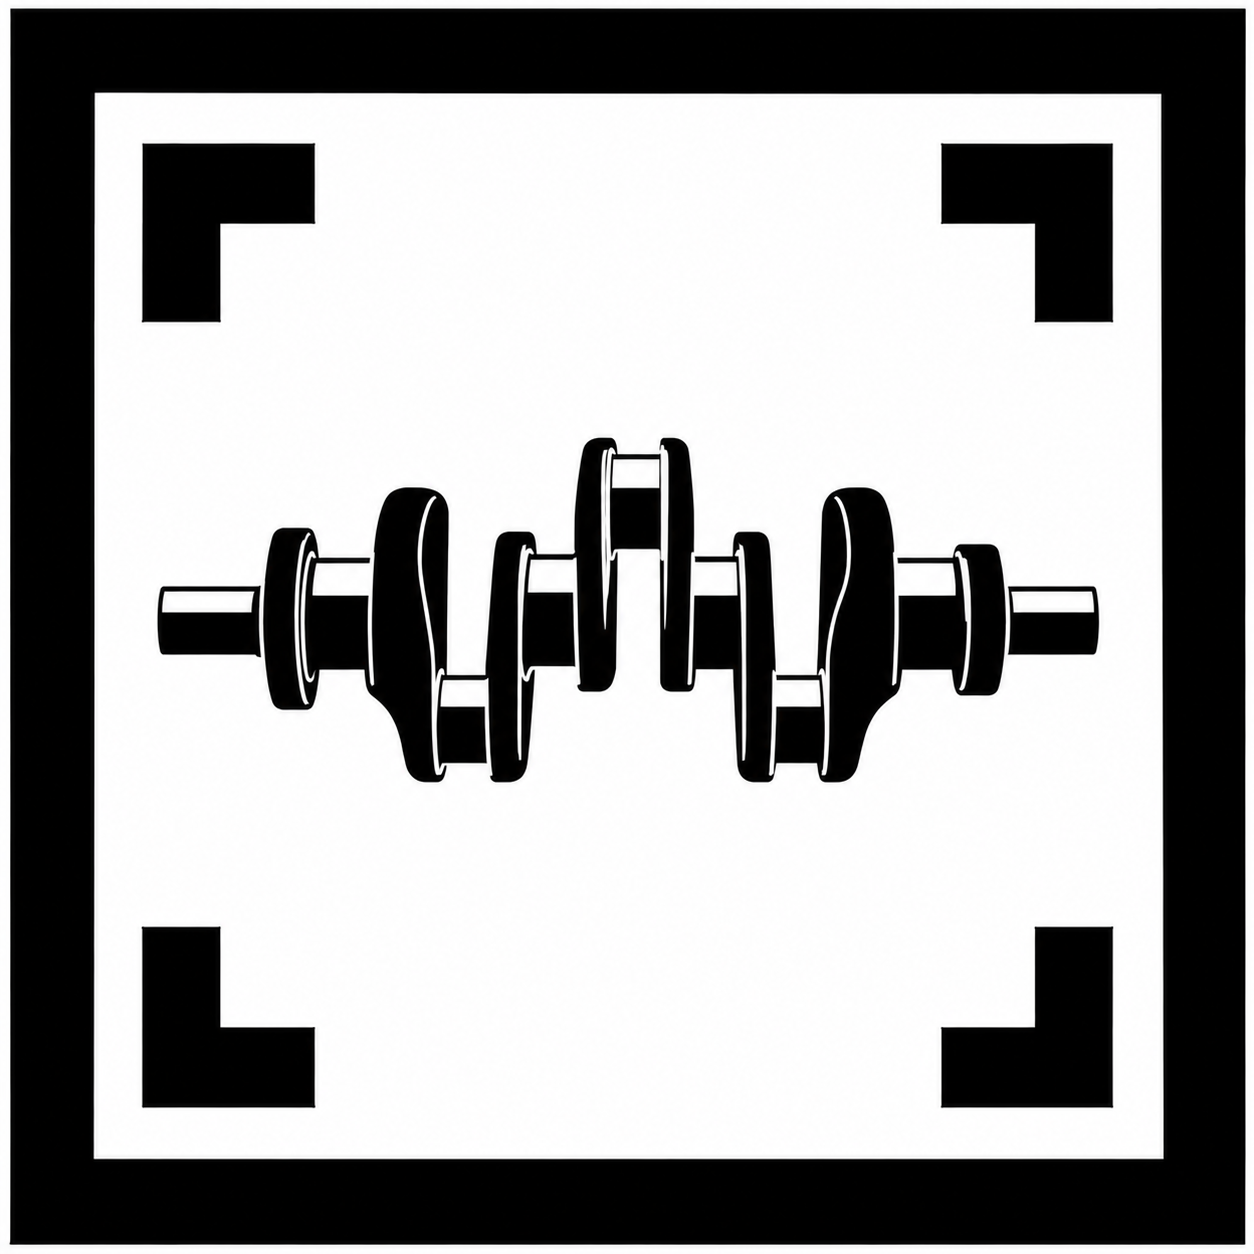
\includegraphics[width=\textwidth]{Assets/Markers/vilebrequin.png}
        \caption{Marqueur Vilebrequin}
    \end{minipage}\hfill
    \begin{minipage}{0.3\textwidth}
        \centering
        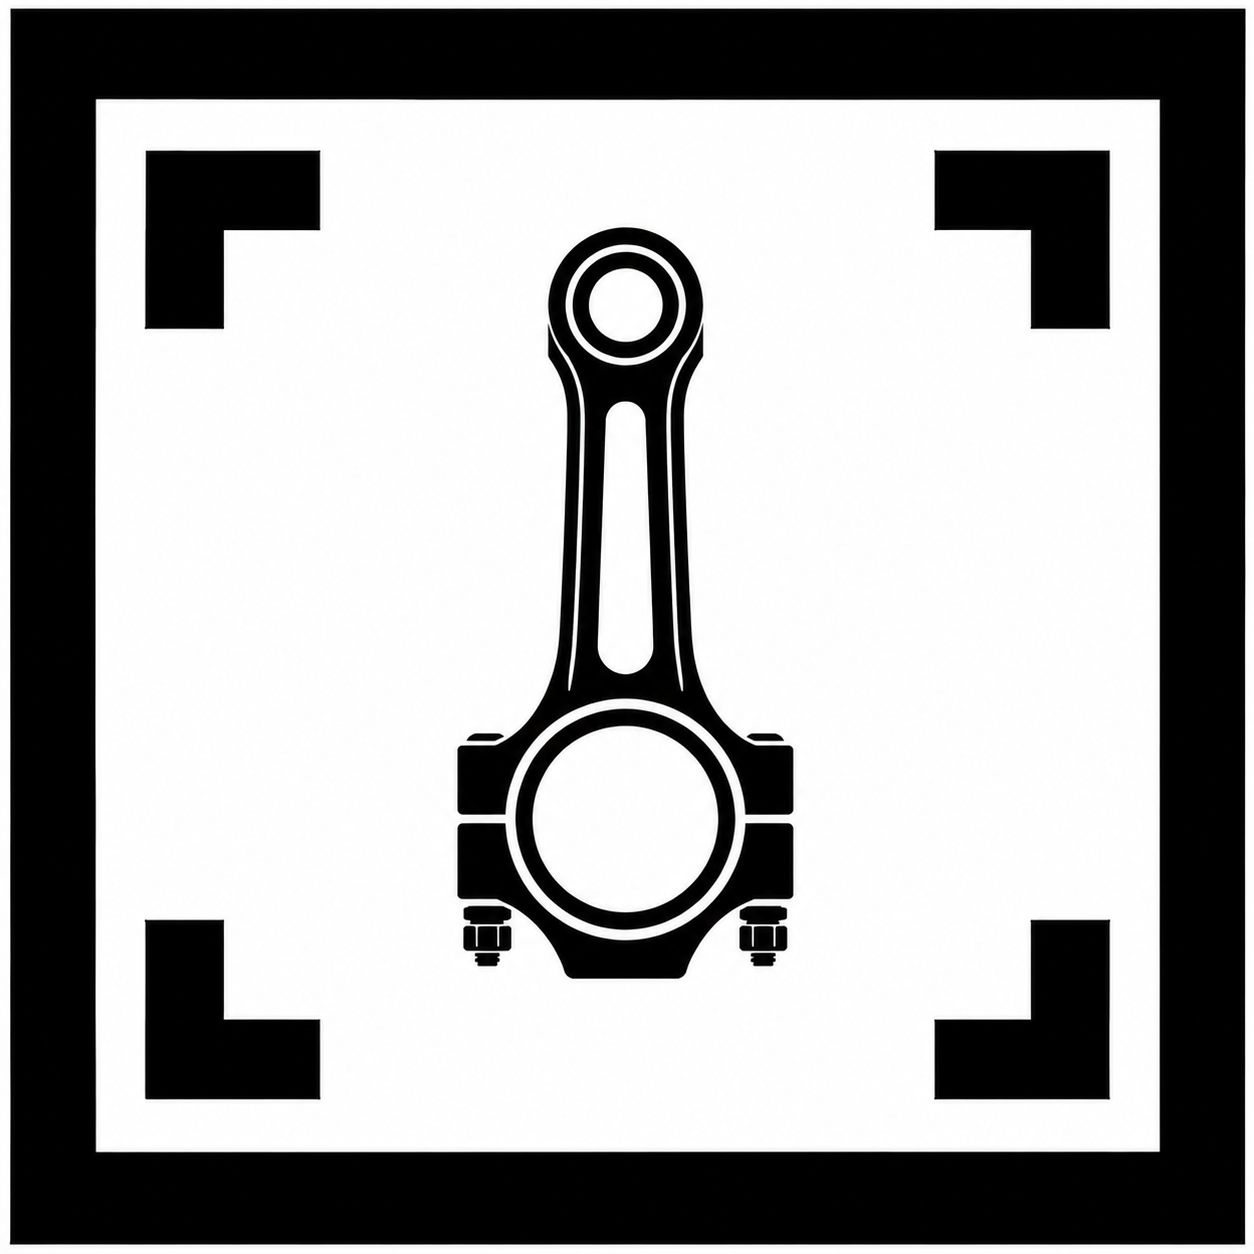
\includegraphics[width=\textwidth]{Assets/Markers/bielle.png}
        \caption{Marqueur Bielle}
    \end{minipage}\hfill
    \begin{minipage}{0.3\textwidth}
        \centering
        
\includegraphics[width=\textwidth]{Assets/Markers/piston.png}
        \caption{Marqueur Piston}
    \end{minipage}
    \label{fig:markers_targets}
\end{figure}

% =========================================================================
\section{Travail Réalisé et Implémentation}
% =========================================================================
Le travail de développement s'est découpé en plusieurs phases d'intégration logicielles et matérielles :

\subsection{Modélisation et Chargement Dynamique de la Procédure}
La séquence de montage est entièrement découplée de la logique de programmation C\#. Un fichier de configuration standardisé en JSON définit dynamiquement la séquence de montage, permettant de modifier les tolérances et les instructions sans recompiler l'application.

Le chargeur de données désérialise le fichier JSON en structures mémoire exploitables par le système de guidage. La structure de données pour chaque étape comprend l'instruction textuelle, le nom du préfabriqué 3D d'annotation à afficher, les coordonnées cibles (position et rotation), les tolérances et le mode de validation.

\subsection{Algorithme de Validation Géométrique Tridimensionnelle}
Le cœur de la validation repose sur un calcul d'écarts géométriques dans l'espace 3D. Deux contrôles distincts sont exécutés en continu ou à la demande :
\begin{enumerate}
    \item \textbf{L'écart de position} : Calculé comme la distance euclidienne en mètres entre la position courante de la pièce suivie et la position théorique définie pour l'étape.
    \[ E_{\text{pos}} = \| \mathbf{P}_{\text{tracked}} - \mathbf{P}_{\text{target}} \| \]
    
    \item \textbf{L'écart d'orientation} : Calculé comme la différence angulaire en degrés entre le quaternion de rotation de l'objet suivi et le quaternion cible.
    \[ E_{\text{rot}} = 2 \arccos(| \mathbf{Q}_{\text{tracked}} \cdot \mathbf{Q}_{\text{target}} |) \times \frac{180}{\pi} \]
\end{enumerate}

Le système accepte la validation si et seulement si les deux écarts sont simultanément inférieurs aux tolérances spécifiées dans l'étape ($E_{\text{pos}} \le \text{tolerance}_{\text{pos}}$ et $E_{\text{rot}} \le \text{tolerance}_{\text{rot}}$).

\subsection{Système d'Évaluation de l'Opérateur}
Pour mesurer l'efficacité du montage, un algorithme d'évaluation a été programmé. Le score de base est fixé à 100 points. Le système applique des pénalités selon le comportement de l'utilisateur :
\begin{itemize}
    \item \textbf{Pénalité d'Erreur} : Une déduction fixe (par défaut 10 points) est appliquée chaque fois que l'opérateur demande une validation alors que la pièce n'est pas correctement positionnée.
    \item \textbf{Pénalité de Temps} : Si le temps moyen passé par étape dépasse une durée de référence (par défaut 60 secondes), une pénalité (5 points par tranche de 30 secondes supplémentaires) est déduite du score final.
\end{itemize}
Une appréciation qualitative finale est calculée en fonction du score obtenu.

\subsection{Interface Utilisateur (HUD) et Guidage Visuel}
L'interface utilisateur a été conçue pour fournir un retour visuel direct et limiter la charge mentale de l'opérateur :
* Un en-tête affiche l'étape en cours et la progression globale (barre de progression).
* Une zone centrale présente l'instruction de montage textuelle.
* Un indicateur de temps dynamique affiche le chronomètre de l'étape.
* Des popups éphémères de couleur verte signalent les validations réussies, tandis que des bandeaux rouges décrivent la cause exacte de l'erreur en cas de mauvaise manipulation (ex: "Position incorrecte de 15 cm").

% =========================================================================
\section{Phase de Tests et de Validation}
% =========================================================================

\subsection{Validation Fonctionnelle dans l'Éditeur Unity}
Pour tester la robustesse géométrique sans nécessiter l'impression immédiate de cibles physiques à chaque itération de développement, des tests ont été réalisés dans l'éditeur Unity à l'aide de la webcam du PC. Les marqueurs affichés sur un écran externe ont été présentés devant l'objectif :
\begin{itemize}
    \item Les modèles d'annotations 3D (flèches de guidage) se positionnent correctement sur les cibles dès leur détection.
    \item En mode `Auto`, la transition à l'étape suivante s'effectue de manière autonome dès que le marqueur entre dans la zone de tolérance.
    \item En mode `Button`, l'interface réagit de manière cohérente, affichant des messages d'erreur détaillant les écarts en centimètres lorsque les tolérances ne sont pas respectées.
\end{itemize}

\subsection{Test du Calcul de Score}
Des scénarios de test d'évaluation ont été déroulés pour s'assurer de la justesse du barème de notation :
\begin{table}[H]
    \centering
    \begin{tabular}{|l|c|c|c|c|}
        \hline
        \textbf{Scénario} & \textbf{Temps Total} & \textbf{Erreurs} & \textbf{Score Calculé} & \textbf{Appréciation} \\
        \hline
        Montage parfait & 180s (36s/étape) & 0 & 100 / 100 & Excellent \\
        Montage ralenti & 350s (70s/étape) & 0 & 95 / 100 & Excellent \\
        Montage avec erreurs & 210s (42s/étape) & 2 & 80 / 100 & Bien \\
        Montage manqué & 420s (84s/étape) & 4 & 55 / 100 & À améliorer \\
        \hline
    \end{tabular}
    \caption{Résultats des tests du système d'évaluation}
    \label{tab:scoring_tests}
\end{table}

% =========================================================================
\section{Conclusion et Perspectives}
% =========================================================================
Le travail accompli a permis d'aboutir à un prototype fonctionnel d'application d'assistance industrielle en Réalité Augmentée. Le découplage des données d'assemblage (JSON) et de la logique de l'application (C\#) offre une grande souplesse pour adapter le système à d'autres cas d'usage industriels.

Les axes d'amélioration identifiés pour de futures versions sont :
\begin{itemize}
    \item \textbf{Transition vers le Model Target 3D} : Utiliser la reconnaissance tridimensionnelle directe des formes CAO des composants réels à la place des marqueurs imprimés en 2D.
    \item \textbf{Interaction Vocale} : Permettre le contrôle de l'avancement ou la validation par des commandes vocales ("Suivant", "Vérifier") afin de laisser les mains de l'opérateur libres pour le travail physique.
    \item \textbf{Portage sur Casque de Réalité Mixte} : Adapter l'interface et le déploiement sur des dispositifs autonomes de type Meta Quest 3 ou Apple Vision Pro pour un confort de travail accru en atelier.
\end{itemize}

\end{document}
